% Multilayer Perceptrons from the Ground Up -- a 20-frame tutorial.
% Build from this directory:   latexmk -pdf mlp_tutorial.tex
% Needs: beamer + metropolis theme, tikz, pgfplots, listings (all in TeX Live).
% Figures read data written by ../experiments.py into generated/;
% frame 18 pulls its listings directly from ../mlp.py and ../train.py.
\documentclass[aspectratio=169,10pt]{beamer}

\usetheme[numbering=fraction,progressbar=frametitle,block=fill]{metropolis}
\geometry{papersize={192mm,108mm}}
\usefonttheme[onlymath]{serif}
\usepackage{amsmath,amssymb,bm,booktabs,array}
\usepackage{tikz,pgfplots,listings}
\pgfplotsset{compat=1.17}
\usetikzlibrary{arrows.meta,positioning,calc,fit,backgrounds,decorations.pathreplacing,matrix}

% ---------------------------------------------------------------- colours
% One colour per stage, used consistently in every diagram.
\definecolor{cInk}{HTML}{22303C}
\definecolor{cTok}{HTML}{5B6770}   % tokens / ids
\definecolor{cEmb}{HTML}{2F6DB5}   % embeddings
\definecolor{cAtt}{HTML}{D9822B}   % attention
\definecolor{cFfn}{HTML}{2E8B57}   % feed-forward
\definecolor{cNrm}{HTML}{8C7A2B}   % normalisation
\definecolor{cOut}{HTML}{7B4FA6}   % output / sampling
\definecolor{cBad}{HTML}{B03A3A}
\setbeamercolor{normal text}{fg=cInk,bg=white}
\setbeamercolor{frametitle}{bg=cInk,fg=white}
\setbeamercolor{progress bar}{fg=cAtt,bg=cAtt!25}
\setbeamercolor{alerted text}{fg=cAtt}
\setbeamercolor{block title}{bg=cEmb!14,fg=cInk}
\setbeamercolor{block body}{bg=cEmb!5}
\setbeamerfont{block title}{series=\bfseries,size=\small}
\setbeamertemplate{itemize item}{\color{cAtt}\rule[0.25ex]{0.9ex}{0.9ex}}
\setbeamertemplate{itemize subitem}{\color{cTok}--}
\setlength{\leftmargini}{1.1em}

% ---------------------------------------------------------------- macros
\newcommand{\R}{\mathbb{R}}
\DeclareMathOperator{\softmax}{softmax}
\DeclareMathOperator{\LN}{LN}
\DeclareMathOperator{\MHA}{MHA}
\DeclareMathOperator{\FFN}{FFN}
\DeclareMathOperator{\Attn}{Attn}
\DeclareMathOperator{\GELU}{GELU}
\newcommand{\T}{\top}
\renewcommand{\cite}[1]{{\scriptsize\color{cTok}[#1]}}
\newcommand{\vsp}{\textvisiblespace}
\newcommand{\key}[1]{\textbf{\color{cAtt}#1}}

\tikzset{
  >={Stealth[length=5pt]},
  stage/.style={draw=#1,fill=#1!12,rounded corners=2pt,line width=0.7pt,
                minimum height=7.5mm,inner xsep=5pt,font=\small,align=center},
  stage/.default=cTok,
  flow/.style={->,line width=0.7pt,draw=cInk!80},
  note/.style={font=\scriptsize,text=cTok,align=center},
  tokbox/.style={draw=cTok,fill=cTok!10,rounded corners=1.5pt,font=\ttfamily\small,
                 minimum height=5.5mm,inner xsep=3pt,outer sep=0pt},
  cell/.style={minimum size=5mm,inner sep=0pt,font=\scriptsize},
}

\lstdefinestyle{py}{
  language=Python,basicstyle=\ttfamily\fontsize{6.1}{7.4}\selectfont,
  keywordstyle=\color{cEmb}\bfseries,commentstyle=\color{cFfn!85!black}\itshape,
  stringstyle=\color{cAtt!85!black},showstringspaces=false,columns=fullflexible,
  keepspaces=true,frame=none,backgroundcolor=\color{cInk!4},
  xleftmargin=3pt,xrightmargin=3pt,aboveskip=2pt,belowskip=2pt,
  literate={-}{{-}}1,
}


\DeclareMathOperator{\ReLU}{ReLU}
\newcommand{\num}[1]{\textbf{\color{cEmb}#1}}

\title{Multilayer Perceptrons from the Ground Up}
\subtitle{Weights, activations, layers, data encoding and the training loop, with runnable code}
\date{A 20-slide tutorial \textbullet{} companion code: \texttt{data.py}, \texttt{mlp\_numpy.py},
      \texttt{mlp.py}, \texttt{train.py}, \texttt{experiments.py}}

\newcommand{\moonsLinearAcc}{87}
\newcommand{\moonsLinearParams}{6}
\newcommand{\moonsMlpAcc}{100}
\newcommand{\moonsMlpParams}{354}
\newcommand{\lrSmallFinal}{0.282}
\newcommand{\lrGoodFinal}{0.088}
\newcommand{\lrNoisyFinal}{0.064}
\newcommand{\lrBrokenFinal}{1.001}
\newcommand{\lrInit}{0.88}
\newcommand{\optSgdLr}{0.1}
\newcommand{\optSgdVal}{0.075}
\newcommand{\optSgdWorst}{0.312}
\newcommand{\optMomentumLr}{0.1}
\newcommand{\optMomentumVal}{0.069}
\newcommand{\optMomentumWorst}{0.129}
\newcommand{\optAdamLr}{0.03}
\newcommand{\optAdamVal}{0.079}
\newcommand{\optAdamWorst}{0.104}
\newcommand{\mpgNtrain}{278}
\newcommand{\bsOneUpdates}{278}
\newcommand{\bsOneMs}{119}
\newcommand{\bsOneVal}{0.087}
\newcommand{\bsEightUpdates}{35}
\newcommand{\bsEightMs}{19}
\newcommand{\bsEightVal}{0.100}
\newcommand{\bsThirtyTwoUpdates}{9}
\newcommand{\bsThirtyTwoMs}{6}
\newcommand{\bsThirtyTwoVal}{0.103}
\newcommand{\bsFullUpdates}{1}
\newcommand{\bsFullMs}{1}
\newcommand{\bsFullVal}{0.138}
\newcommand{\ofParams}{70{,}402}
\newcommand{\ofBestEpoch}{2}
\newcommand{\ofBestVal}{0.482}
\newcommand{\ofLastVal}{1.310}
\newcommand{\ofLastTrain}{0.156}
\newcommand{\ofLastAcc}{83.0}
\newcommand{\ofStoppedAcc}{85.2}
\newcommand{\titanicMlpParams}{1634}
\newcommand{\titanicMlpEpochs}{46}
\newcommand{\cmTN}{77}
\newcommand{\cmFP}{7}
\newcommand{\cmFN}{12}
\newcommand{\cmTP}{39}
\newcommand{\titanicSeedAcc}{85.9}
\newcommand{\titanicBaseAcc}{62.2}
\newcommand{\titanicNtest}{135}
\newcommand{\titanicNfeat}{15}
\newcommand{\titanicMlpMean}{81.6}
\newcommand{\titanicMlpStd}{2.9}
\newcommand{\titanicLinearParams}{32}
\newcommand{\titanicLinearEpochs}{70}
\newcommand{\titanicLinearMean}{82.7}
\newcommand{\titanicLinearStd}{2.4}
\newcommand{\mpgMlpParams}{1441}
\newcommand{\mpgMlpEpochs}{105}
\newcommand{\mpgSeedRmse}{2.84}
\newcommand{\mpgSeedMae}{1.95}
\newcommand{\mpgSeedRsq}{0.83}
\newcommand{\mpgBaseRmse}{6.87}
\newcommand{\mpgNtest}{61}
\newcommand{\mpgNfeat}{10}
\newcommand{\mpgMlpMean}{2.95}
\newcommand{\mpgMlpStd}{0.75}
\newcommand{\mpgLinearParams}{11}
\newcommand{\mpgLinearEpochs}{127}
\newcommand{\mpgLinearMean}{3.29}
\newcommand{\mpgLinearStd}{0.41}
\newcommand{\titanicMlpBetter}{3}
\newcommand{\titanicTies}{1}
\newcommand{\mpgMlpBetter}{7}

\begin{document}

% ======================================================================= 1
\maketitle
\addtocounter{framenumber}{1}

% ======================================================================= 2
\begin{frame}{The big picture: a trainable function from inputs to outputs}
\begin{columns}[T,onlytextwidth]
\column{0.50\textwidth}
\small
\textbf{Supervised learning}: we have examples $(x, y)$, an input and the known correct answer,
and want a function $f_\theta$ with $f_\theta(x)\approx y$ that also works on \emph{new} inputs.

\vspace{1mm}
A \key{multilayer perceptron} (MLP) is the simplest neural network for this job:
layers of simple units (``neurons''), each layer feeding the next.
$\theta$ is the collection of all its \textbf{weights}; \emph{training} means adjusting
$\theta$ until the outputs match the answers.
\column{0.46\textwidth}
\begin{block}{Two real problems used throughout}
\footnotesize
\begin{itemize}
  \item \textbf{Classification}: Titanic passenger list, 891 rows. Did this passenger survive?
        (yes / no)
  \item \textbf{Regression}: Auto MPG, 398 cars. How many miles per gallon does this car get?
        (a number)
\end{itemize}
\end{block}
\end{columns}
\vspace{2mm}
\centering
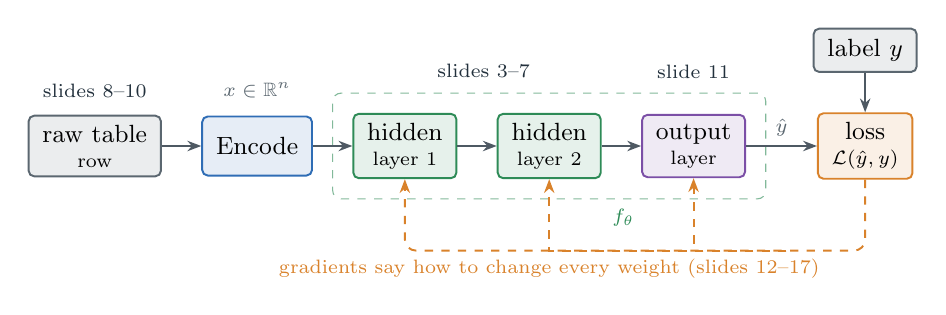
\begin{tikzpicture}[node distance=5mm]
  \node[stage=cTok] (raw) {raw table\\[-2pt]{\scriptsize row}};
  \node[stage=cEmb,right=of raw] (enc) {Encode};
  \node[stage=cFfn,right=of enc] (h1) {hidden\\[-2pt]{\scriptsize layer 1}};
  \node[stage=cFfn,right=of h1] (h2) {hidden\\[-2pt]{\scriptsize layer 2}};
  \node[stage=cOut,right=of h2] (out) {output\\[-2pt]{\scriptsize layer}};
  \node[stage=cAtt,right=9mm of out] (loss) {loss\\[-2pt]{\scriptsize $\mathcal L(\hat y, y)$}};
  \node[stage=cTok,above=5mm of loss,minimum height=5.5mm] (lab) {label $y$};
  \draw[flow] (raw)--(enc); \draw[flow] (enc)--(h1); \draw[flow] (h1)--(h2); \draw[flow] (h2)--(out);
  \draw[flow] (out)-- node[above,note]{$\hat y$} (loss); \draw[flow] (lab)--(loss);
  \draw[flow,dashed,cAtt,rounded corners=4pt] (loss.south) |- ++(-10mm,-9mm) -| (h1.south);
  \draw[flow,dashed,cAtt] ($(loss.south)+(-10mm,-9mm)$) -| (h2.south);
  \draw[flow,dashed,cAtt] ($(loss.south)+(-10mm,-9mm)$) -| (out.south);
  \node[note,text=cAtt] at ($(h2.south)+(0,-11.3mm)$) {gradients say how to change every weight (slides 12--17)};
  \node[note,above=1mm of enc] {$x\in\R^{n}$};
  \node[note,above=1mm of raw,text=cInk] {slides 8--10};
  \node[note,above=3.2mm of h1,xshift=10mm,text=cInk] {slides 3--7};
  \node[note,above=3.2mm of out,text=cInk] {slide 11};
  \begin{scope}[on background layer]
    \node[draw=cFfn!60,dashed,rounded corners=3pt,fit=(h1)(out),inner sep=2.5mm,label={[note,text=cFfn]below right:$f_\theta$}] {};
  \end{scope}
\end{tikzpicture}
\end{frame}

% ======================================================================= 3
\begin{frame}{The neuron: weights, bias, activation}
\begin{columns}[T,onlytextwidth]
\column{0.42\textwidth}
\centering
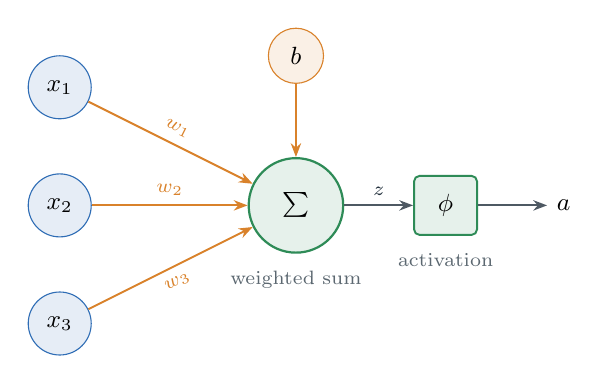
\begin{tikzpicture}[font=\small]
  \foreach \i/\y in {1/1.5,2/0,3/-1.5}
    \node[circle,draw=cEmb,fill=cEmb!12,minimum size=8mm,inner sep=0pt] (x\i) at (0,\y) {$x_\i$};
  \node[circle,draw=cFfn,fill=cFfn!12,minimum size=12mm,line width=0.8pt] (s) at (3.0,0) {$\sum$};
  \node[stage=cFfn,minimum width=8mm] (phi) at (4.9,0) {$\phi$};
  \node (a) at (6.4,0) {$a$};
  \node[circle,draw=cAtt,fill=cAtt!12,minimum size=7mm,inner sep=0pt] (b) at (3.0,1.9) {$b$};
  \foreach \i/\p in {1/above,2/above,3/below}
    \draw[flow,cAtt] (x\i) -- node[\p,sloped,text=cAtt,font=\scriptsize] {$w_\i$} (s);
  \draw[flow,cAtt] (b)--(s);
  \draw[flow] (s)-- node[above,note,text=cInk]{$z$} (phi); \draw[flow] (phi)--(a);
  \node[note,below=1mm of s] {weighted sum};
  \node[note,below=1mm of phi] {activation};
\end{tikzpicture}
\[
  z=\sum_i w_i x_i+b=w\cdot x+b,\qquad a=\phi(z)
\]
\vspace{-2mm}
\begin{block}{By hand}
\footnotesize
$x=(2,\,1)$,\ \ $w=(0.5,\,-1)$,\ \ $b=0.5$:\\[1mm]
$z=0.5\cdot2+(-1)\cdot1+0.5=\num{0.5}$\\[1mm]
$\ReLU(z)=0.5$,\quad sigmoid$(z)=0.622$,\quad $\tanh(z)=0.462$
\end{block}
\column{0.55\textwidth}
\small
\begin{itemize}
  \item A \key{weight} $w_i$ says how much input $i$ matters and in which direction:
        positive pushes the output up, negative pushes it down, zero ignores the input.
  \item The \key{bias} $b$ shifts the threshold: the neuron's output when all inputs are zero.
  \item The \key{activation function} $\phi$ bends the result (next slide).
  \item \textbf{Geometry}: $w\cdot x+b=0$ is a line (in general a hyperplane). The neuron
        asks ``which side of this boundary is $x$ on, and how far?''
  \item \textbf{Weights are the only thing that learns.} They start as small random numbers;
        training changes them. ``A model with 1{,}634 parameters'' means 1{,}634 such numbers.
  \item One neuron alone is the \emph{perceptron} of the 1950s \cite{1}. It can only separate
        classes with a single straight boundary, which is why we need layers.
\end{itemize}
\end{columns}
\end{frame}

% ======================================================================= 4
\begin{frame}{Activation functions: where the nonlinearity comes from}
\begin{columns}[T,onlytextwidth]
\column{0.44\textwidth}
\centering
\begin{tikzpicture}
\begin{axis}[width=7.6cm,height=5.0cm,axis lines=left,xmin=-5,xmax=5,ymin=-1.15,ymax=3.1,
  grid=major,grid style={cInk!10},xtick={-4,-2,0,2,4},ytick={-1,0,1,2,3},tick label style={font=\tiny},
  legend style={font=\scriptsize,draw=none,fill=none,at={(0.03,0.98)},anchor=north west},legend cell align=left,
  every axis plot/.append style={line width=1.1pt,no marks}]
  \addplot[cFfn] table[x=x,y=relu]{generated/act.dat}; \addlegendentry{ReLU}
  \addplot[cAtt,dashed] table[x=x,y=tanh]{generated/act.dat}; \addlegendentry{tanh}
  \addplot[cOut,densely dotted] table[x=x,y=sigmoid]{generated/act.dat}; \addlegendentry{sigmoid}
\end{axis}
\end{tikzpicture}

{\footnotesize
\renewcommand{\arraystretch}{1.25}
\begin{tabular}{@{}llll@{}}
\toprule
 & $\phi(z)$ & range & $\phi'(z)$\\
\midrule
ReLU & $\max(0,z)$ & $[0,\infty)$ & $1$ if $z>0$ else $0$\\
tanh & $\tanh z$ & $(-1,1)$ & $1-\tanh^2 z\ \le 1$\\
sigmoid & $1/(1+e^{-z})$ & $(0,1)$ & $\sigma(1-\sigma)\ \le \tfrac14$\\
\bottomrule
\end{tabular}}
\column{0.53\textwidth}
\small
\key{Why not skip it?} Without $\phi$, two layers collapse into one:
\[
  (xW_1)W_2=x\,(W_1W_2)=xW .
\]
A stack of linear layers is still a linear model, however deep. The nonlinearity is what
lets layers build something new on top of each other.

\vspace{1mm}
\key{Which one?}
\begin{itemize}
  \item \textbf{Hidden layers: ReLU} by default \cite{6}. Cheap, and its slope is exactly 1
        for active units, so gradients pass through many layers undiminished.
  \item \textbf{Sigmoid and tanh saturate}: for large $|z|$ the slope is nearly 0 and learning
        stalls (``vanishing gradients''). Sigmoid's slope is never above $\tfrac14$.
  \item \textbf{Output layer}: chosen by the task, not by taste. None for regression;
        sigmoid or softmax for classification (slide 11).
\end{itemize}
A ReLU unit with $z<0$ outputs 0 and gets no gradient: it is ``off'' for that input.
\end{columns}
\end{frame}

% ======================================================================= 5
\begin{frame}{Layers: many neurons at once, written as matrices}
\begin{columns}[T,onlytextwidth]
\column{0.47\textwidth}
\centering
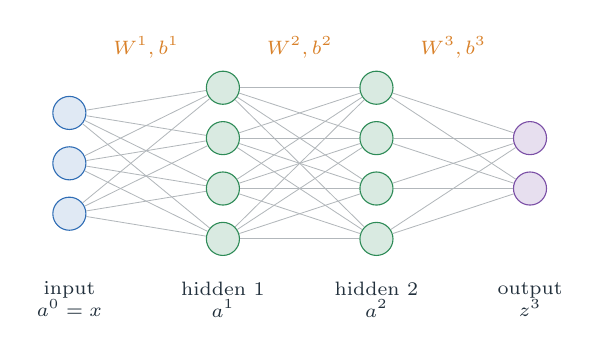
\begin{tikzpicture}[x=13mm,y=6.4mm]
  \foreach \i in {1,2,3} \node[circle,draw=cEmb,fill=cEmb!15,minimum size=4.2mm,inner sep=0] (a\i) at (0,\i-2) {};
  \foreach \i in {1,...,4} \node[circle,draw=cFfn,fill=cFfn!18,minimum size=4.2mm,inner sep=0] (b\i) at (1.5,\i-2.5) {};
  \foreach \i in {1,...,4} \node[circle,draw=cFfn,fill=cFfn!18,minimum size=4.2mm,inner sep=0] (c\i) at (3,\i-2.5) {};
  \foreach \i in {1,2} \node[circle,draw=cOut,fill=cOut!18,minimum size=4.2mm,inner sep=0] (d\i) at (4.5,\i-1.5) {};
  \foreach \i in {1,2,3} \foreach \j in {1,...,4} \draw[cInk!35,line width=0.3pt] (a\i)--(b\j);
  \foreach \i in {1,...,4} \foreach \j in {1,...,4} \draw[cInk!35,line width=0.3pt] (b\i)--(c\j);
  \foreach \i in {1,...,4} \foreach \j in {1,2} \draw[cInk!35,line width=0.3pt] (c\i)--(d\j);
  \node[note,text=cAtt] at (0.75,2.3) {$W^1,b^1$}; \node[note,text=cAtt] at (2.25,2.3) {$W^2,b^2$};
  \node[note,text=cAtt] at (3.75,2.3) {$W^3,b^3$};
  \node[note,text=cInk] at (0,-2.7) {input\\$a^0=x$}; \node[note,text=cInk] at (1.5,-2.7) {hidden 1\\$a^1$};
  \node[note,text=cInk] at (3,-2.7) {hidden 2\\$a^2$}; \node[note,text=cInk] at (4.5,-2.7) {output\\$z^3$};
\end{tikzpicture}

\vspace{1mm}
\begin{block}{Forward pass, layer $\ell=1..L$}
\vspace{-2mm}
\[
  a^0=x,\qquad z^{\ell}=a^{\ell-1}W^{\ell}+b^{\ell},\qquad a^{\ell}=\phi(z^{\ell})
\]
\footnotesize The last layer has no $\phi$: its raw output $z^L$ goes to the loss.
\end{block}
\column{0.50\textwidth}
\small
\begin{itemize}
  \item A \key{layer} is a set of neurons that all read the same inputs. Stack their weight
        vectors as the columns of one matrix: $W^{\ell}\in\R^{n_{\ell-1}\times n_\ell}$.
  \item \textbf{Fully connected} (``dense''): every neuron sees every output of the layer before.
  \item \textbf{Hidden} layers are the ones between input and output. \textbf{Depth} = number of
        layers; \textbf{width} = neurons per layer.
  \item A whole batch at once: rows of $X\in\R^{B\times n_0}$ are examples, and the same formula
        $XW+b$ handles all $B$ of them in one matrix product.
\end{itemize}
\textbf{Counting parameters}: layer $\ell$ has $(n_{\ell-1}+1)\,n_\ell$.
Our Titanic network $15\to32\to32\to2$:
\[
  16\cdot32+33\cdot32+33\cdot2=512+1056+66=\num{1{,}634}.
\]
\key{Initialisation.} All-zero weights would make every neuron in a layer identical forever.
Start random, scaled to the layer: $W^{\ell}_{ij}\sim\mathcal N(0,\,2/n_{\ell-1})$, $b=0$
(``He'' initialisation, for ReLU \cite{8}; \cite{7} for tanh).
\end{columns}
\end{frame}

% ======================================================================= 6
\begin{frame}{Why hidden layers? A problem no straight line can solve}
\begin{columns}[T,onlytextwidth]
\column{0.58\textwidth}
\centering
\begin{tikzpicture}
\begin{axis}[name=lin,width=5.5cm,height=4.7cm,xmin=-1.6,xmax=2.6,ymin=-1.2,ymax=1.7,
  ticks=none,axis line style={cInk!40},title={\scriptsize no hidden layer: \moonsLinearAcc\% on test},
  title style={yshift=-1.5mm}]
  \addplot[only marks,mark size=0.9pt,cEmb,restrict expr to domain={\thisrow{label}}{0:0}] table[x=x,y=y]{generated/moons_points.dat};
  \addplot[only marks,mark size=0.9pt,cAtt,mark=square*,restrict expr to domain={\thisrow{label}}{1:1}] table[x=x,y=y]{generated/moons_points.dat};
  \addplot[cInk,line width=1.3pt,no marks,empty line=jump] table[x=x,y=y]{generated/moons_linear.dat};
\end{axis}
\begin{axis}[at={(lin.east)},anchor=west,xshift=7mm,width=5.5cm,height=4.7cm,xmin=-1.6,xmax=2.6,ymin=-1.2,ymax=1.7,
  ticks=none,axis line style={cInk!40},title={\scriptsize hidden layers 16, 16: \moonsMlpAcc\% on test},
  title style={yshift=-1.5mm}]
  \addplot[only marks,mark size=0.9pt,cEmb,restrict expr to domain={\thisrow{label}}{0:0}] table[x=x,y=y]{generated/moons_points.dat};
  \addplot[only marks,mark size=0.9pt,cAtt,mark=square*,restrict expr to domain={\thisrow{label}}{1:1}] table[x=x,y=y]{generated/moons_points.dat};
  \addplot[cInk,line width=1.3pt,no marks,empty line=jump] table[x=x,y=y]{generated/moons_mlp.dat};
\end{axis}
\end{tikzpicture}

\vspace{0.5mm}
{\scriptsize\color{cTok}``Two moons'' toy data (220 training points shown). Black curve: where the trained model
switches class. Both trained by \texttt{experiments.py}; 90 held-out test points.}

\vspace{1.5mm}
\raggedright\small
The left model has \moonsLinearParams{} parameters, the right one \moonsMlpParams. The data and the
training procedure are identical; only the hidden layers differ.
\column{0.39\textwidth}
\small
\begin{itemize}
  \item Each first-layer ReLU neuron contributes \textbf{one straight fold} in the input plane.
  \item The next layer \textbf{combines folds} into bent regions; more layers combine those.
  \item So hidden layers \emph{learn features}: new coordinates in which the problem becomes
        easy for the final layer.
\end{itemize}
\begin{block}{Universal approximation \cite{4,5}}
\footnotesize
One hidden layer with enough neurons can approximate any continuous function on a bounded region
as closely as you like. It says a good set of weights \emph{exists}; it does not say how many
neurons you need or that training will find them.
\end{block}
{\footnotesize The classic case is XOR, which no single neuron can compute \cite{2};
\texttt{mlp\_numpy.py} learns it with 8 hidden units.}
\end{columns}
\end{frame}

% ======================================================================= 7
\begin{frame}{A forward pass by hand}
\begin{columns}[T,onlytextwidth]
\column{0.52\textwidth}
\centering
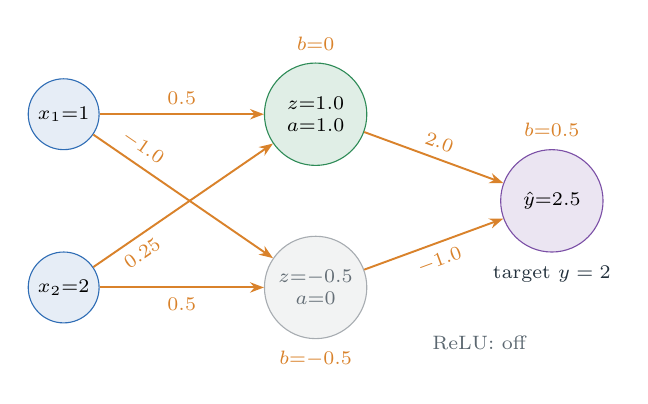
\begin{tikzpicture}[font=\scriptsize,x=10mm,y=10mm]
  \node[circle,draw=cEmb,fill=cEmb!12,minimum size=9mm,inner sep=0] (x1) at (0,1.1) {$x_1{=}1$};
  \node[circle,draw=cEmb,fill=cEmb!12,minimum size=9mm,inner sep=0] (x2) at (0,-1.1) {$x_2{=}2$};
  \node[circle,draw=cFfn,fill=cFfn!15,minimum size=13mm,inner sep=0,align=center] (h1) at (3.2,1.1) {$z{=}1.0$\\$a{=}1.0$};
  \node[circle,draw=cInk!40,fill=cInk!6,minimum size=13mm,inner sep=0,align=center,text=cInk!70] (h2) at (3.2,-1.1) {$z{=}{-}0.5$\\$a{=}0$};
  \node[circle,draw=cOut,fill=cOut!15,minimum size=13mm,inner sep=0,align=center] (o) at (6.2,0) {$\hat y{=}2.5$};
  \draw[flow,cAtt] (x1)-- node[above,text=cAtt]{$0.5$} (h1);
  \draw[flow,cAtt] (x1)-- node[pos=0.22,above,sloped,text=cAtt]{$-1.0$} (h2);
  \draw[flow,cAtt] (x2)-- node[pos=0.22,below,sloped,text=cAtt]{$0.25$} (h1);
  \draw[flow,cAtt] (x2)-- node[below,text=cAtt]{$0.5$} (h2);
  \draw[flow,cAtt] (h1)-- node[above,sloped,text=cAtt]{$2.0$} (o);
  \draw[flow,cAtt] (h2)-- node[below,sloped,text=cAtt]{$-1.0$} (o);
  \node[note,text=cAtt,above=0.3mm of h1] {$b{=}0$}; \node[note,text=cAtt,below=0.3mm of h2] {$b{=}{-}0.5$};
  \node[note,text=cAtt,above=0.3mm of o] {$b{=}0.5$};
  \node[note,below=0.5mm of o,text=cInk] {target $y=2$};
  \node[note,right=-1mm of h2,xshift=8mm,yshift=-7mm] {ReLU: off};
\end{tikzpicture}

\vspace{1mm}
{\footnotesize\color{cTok}A $2\to2\to1$ regression network. Orange numbers are weights and biases.}
\column{0.45\textwidth}
\small
\textbf{Layer 1} \ ($z^1=xW^1+b^1$, then ReLU)
\vspace{-1mm}
\begin{align*}
 z^1_1 &= 1(0.5)+2(0.25)+0 = \num{1.0} &&\Rightarrow a^1_1=1.0\\
 z^1_2 &= 1(-1.0)+2(0.5)-0.5 = \num{-0.5} &&\Rightarrow a^1_2=0
\end{align*}
\vspace{-5mm}

\textbf{Output layer} \ (no activation)
\vspace{-1mm}
\[
 \hat y = 1.0(2.0)+0(-1.0)+0.5=\num{2.5}
\]
\vspace{-4mm}

\textbf{Loss} \ (squared error)
\vspace{-1mm}
\[
 \mathcal L=(\hat y-y)^2=(2.5-2)^2=\num{0.25}
\]
\vspace{-4mm}
\begin{block}{What to notice}
\footnotesize
\begin{itemize}
  \item Prediction is nothing but multiply, add, clip at zero.
  \item The second hidden neuron is switched off for this input: it contributes nothing to $\hat y$.
  \item The loss turns ``how wrong?'' into one number. Slide 13 uses it to correct the weights.
\end{itemize}
\end{block}
\end{columns}
\end{frame}

% ======================================================================= 8
\begin{frame}{Input data I: numerical columns}
\begin{columns}[T,onlytextwidth]
\column{0.50\textwidth}
\small
A network multiplies inputs by weights, so \textbf{the size of a number matters}. Raw columns
arrive on wildly different scales:

\vspace{1mm}
{\footnotesize
\begin{tabular}{@{}llr@{}}
\toprule
column & meaning & typical values\\
\midrule
\texttt{age} & years & 0.4 \dots{} 80\\
\texttt{fare} & ticket price (\pounds) & 0 \dots{} 512\\
\texttt{weight} & car weight (lb) & 1{,}600 \dots{} 5{,}100\\
\texttt{sibsp} & siblings/spouses aboard & 0 \dots{} 8\\
\bottomrule
\end{tabular}}

\vspace{2mm}
\key{Standardise} every numerical column:
\[
  x'=\frac{x-\mu}{\sigma}
\]
with $\mu,\sigma$ the mean and standard deviation of that column. After this each column has mean 0 and spread 1, so one learning rate suits all weights and
training converges far more reliably \cite{9}.

\vspace{1mm}
{\footnotesize Example: the training split has $\mu_\text{age}=29.76$, $\sigma_\text{age}=14.77$, so a
32-year-old becomes $(32-29.76)/14.77=\num{0.151}$.}
\column{0.47\textwidth}
\small
\begin{block}{Skewed columns: take a logarithm first}
\footnotesize
Fares: minimum 0, median 15.05, maximum 512.33. A few huge values would dominate.
Use $\ln(1+x)$, then standardise:
\[
 7.75\;\to\;\ln 8.75=2.169\;\to\;\frac{2.169-2.986}{0.958}=\num{-0.853}
\]
\end{block}
\begin{block}{Rule: statistics come from the training split only}
\footnotesize
Compute $\mu$ and $\sigma$ on training rows, then reuse those same numbers for validation, test
and future data. Otherwise information about the test set leaks into training
(\texttt{TabularEncoder.fit} / \texttt{.transform} in \texttt{data.py}).
\end{block}
\begin{itemize}\footnotesize
  \item Counts and integers (\texttt{sibsp}, \texttt{cylinders}) are numerical too.
  \item Identifiers (name, ticket number) are \emph{not} features: drop them.
  \item Alternative scaling: min--max to $[0,1]$. Fine for bounded data, fragile with outliers.
\end{itemize}
\end{columns}
\end{frame}

% ======================================================================= 9
\begin{frame}{Input data II: logical, categorical and missing values}
\centering
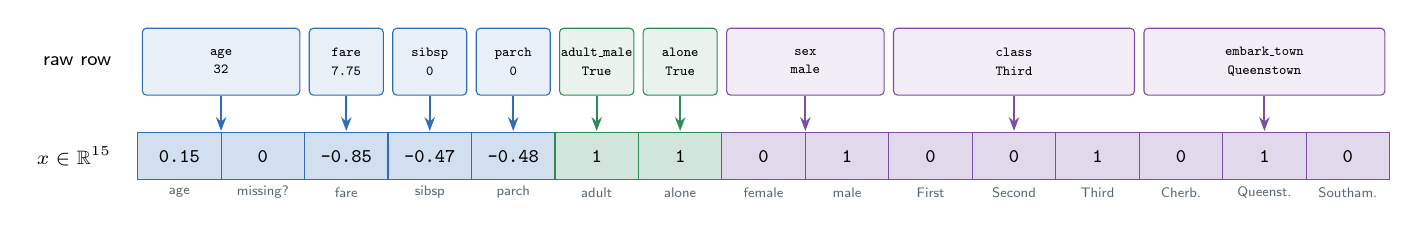
\begin{tikzpicture}[x=10.6mm,y=1mm,font=\ttfamily\scriptsize]
  % groups: name / raw value / first cell index / number of cells / colour
  \foreach \name/\raw/\s/\n/\c in {age/32/0/2/cEmb,fare/7.75/2/1/cEmb,sibsp/0/3/1/cEmb,parch/0/4/1/cEmb,
      adult\_male/True/5/1/cFfn,alone/True/6/1/cFfn,sex/male/7/2/cOut,class/Third/9/3/cOut,embark\_town/Queenstown/12/3/cOut} {
    \node[draw=\c,fill=\c!10,rounded corners=1.5pt,minimum height=8.5mm,minimum width=\n*10.6mm-1.2mm,inner sep=0.5pt,align=center,font=\ttfamily\fontsize{5.4}{6.6}\selectfont]
      (r\s) at (\s+\n/2,14) {\name\\\raw};
    \draw[flow,\c] (r\s.south) -- (\s+\n/2,5.2);
  }
  \foreach \i/\v/\c in {0/0.15/cEmb,1/0/cEmb,2/-0.85/cEmb,3/-0.47/cEmb,4/-0.48/cEmb,5/1/cFfn,6/1/cFfn,
      7/0/cOut,8/1/cOut,9/0/cOut,10/0/cOut,11/1/cOut,12/0/cOut,13/1/cOut,14/0/cOut}
    \node[draw=\c,fill=\c!22,minimum height=6mm,minimum width=10.6mm,inner sep=0pt] at (\i+0.5,2) {\v};
  \foreach \i/\t in {0/age,1/missing?,2/fare,3/sibsp,4/parch,5/adult,6/alone,7/female,8/male,9/First,10/Second,11/Third,12/Cherb.,13/Queenst.,14/Southam.}
    \node[font=\fontsize{4.8}{5}\selectfont\sffamily,text=cTok] at (\i+0.5,-2.6) {\t};
  \node[font=\scriptsize\sffamily,anchor=east] at (-0.2,14) {raw row}; \node[font=\scriptsize\sffamily,anchor=east] at (-0.2,2) {$x\in\R^{15}$};
\end{tikzpicture}

\vspace{1.5mm}
\begin{columns}[T,onlytextwidth]
\column{0.32\textwidth}
\begin{block}{\color{cFfn!70!black}Logical (true/false)}
\footnotesize
Map False $\to0$, True $\to1$. Already on a good scale; no standardising needed.
\end{block}
\begin{block}{\color{cEmb}Missing values}
\footnotesize
134 of 623 training ages are blank. Fill with the mean (which is 0 after standardising) and add
a 0/1 column ``was missing'', so the network can tell a real average from a gap.
\end{block}
\column{0.32\textwidth}
\begin{block}{\color{cOut}Categorical (one of $K$ names)}
\footnotesize
\textbf{One-hot}: $K$ columns, a single 1 marking the category.
\texttt{class=Third} $\to(0,0,1)$.

\vspace{1mm}
A category never seen in training becomes all zeros.
\end{block}
\column{0.32\textwidth}
\begin{block}{Do not number unordered categories}
\footnotesize
Coding Cherbourg $=0$, Queenstown $=1$, Southampton $=2$ tells the network that Queenstown lies
``between'' the others and that Southampton is ``twice'' Queenstown. Neither is true.
\end{block}
{\footnotesize Truly ordered categories (small/medium/large) may use integers. Columns with
thousands of categories use learned \emph{embeddings} instead of one-hot.}
\end{columns}
\end{frame}

% ====================================================================== 10
\begin{frame}{Labeled data: answers, encodings and the three splits}
\begin{columns}[T,onlytextwidth]
\column{0.49\textwidth}
\small
A \key{label} is the known correct answer attached to an example. Labels come from records,
measurements or human annotators, and the model can never be more reliable than they are.

\vspace{1mm}
\begin{block}{Encoding the label}
\footnotesize
\begin{itemize}
  \item \textbf{Classification}: class names $\to$ integer ids. \texttt{no} $\to0$, \texttt{yes} $\to1$.
        With $K$ classes the network gets $K$ outputs, one score per class. The ids are only
        names for the outputs; the loss treats them as one-hot vectors.
  \item \textbf{Regression}: the label is a number (mpg). Standardise it like an input, train on
        the standardised value, convert predictions back to real units for reporting.
\end{itemize}
\end{block}
\begin{block}{Always compare with a trivial baseline}
\footnotesize
\titanicBaseAcc\% of our Titanic test passengers died, so ``always answer \texttt{no}'' already scores
\titanicBaseAcc\% accuracy. A model must beat that to have learned anything.
\end{block}
\column{0.48\textwidth}
\centering
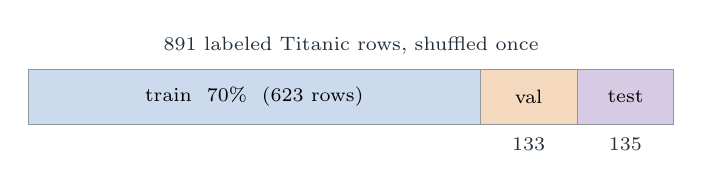
\begin{tikzpicture}[x=0.82mm,y=1mm,font=\scriptsize]
  \fill[cEmb!25] (0,0) rectangle (70,7); \fill[cAtt!30] (70,0) rectangle (85,7); \fill[cOut!30] (85,0) rectangle (100,7);
  \draw[cInk!50] (0,0) rectangle (100,7); \draw[cInk!50] (70,0)--(70,7) (85,0)--(85,7);
  \node at (35,3.5) {train \ 70\% \ (623 rows)}; \node at (77.5,3.5) {val}; \node at (92.5,3.5) {test};
  \node[note,text=cInk] at (77.5,-2.5) {133}; \node[note,text=cInk] at (92.5,-2.5) {135};
  \node[note,text=cInk] at (50,10) {891 labeled Titanic rows, shuffled once};
\end{tikzpicture}

\vspace{1mm}
\raggedright\small
{\footnotesize
\renewcommand{\arraystretch}{1.2}
\begin{tabular}{@{}lp{58mm}@{}}
\toprule
\textbf{train} & the only rows that change the weights\\
\textbf{validation} & watched during training: when to stop, which learning rate or network size to keep\\
\textbf{test} & used once, at the end, for the number you report\\
\bottomrule
\end{tabular}}

\vspace{1.5mm}
\key{Leakage}: any path by which the answer sneaks into the input.
\begin{itemize}\footnotesize
  \item The Titanic file has a column \texttt{survived} that duplicates the label \texttt{alive}.
        Feed it in and you get 100\% accuracy and a useless model.
  \item Tuning choices on the test set makes the test score optimistic. That is what the
        validation set is for.
\end{itemize}
\end{columns}
\end{frame}

% ====================================================================== 11
\begin{frame}{The output layer and the loss: regression vs.\ classification}
\small
The hidden layers are the same for both tasks. Only the last layer and the loss change:

\vspace{1mm}
{\footnotesize
\renewcommand{\arraystretch}{1.3}
\begin{tabular}{@{}p{26mm}p{66mm}p{70mm}@{}}
\toprule
 & \textbf{Regression} (predict a number) & \textbf{Classification} (predict one of $K$ classes)\\
\midrule
output neurons & 1 & $K$ \ (scores called \emph{logits}, $z_1..z_K$)\\
output activation & none: $\hat y=z$ & softmax: $p_k=e^{z_k}/\sum_j e^{z_j}$, \ positive, sums to 1\\
loss (mean over batch) & squared error \ $(\hat y-y)^2$ \ (MSE) & cross-entropy \ $-\ln p_{y}$ \ (probability given to the true class)\\
prediction & $\hat y$ & $\arg\max_k p_k$\\
report & RMSE, MAE, $R^2$ & accuracy, confusion matrix, precision/recall\\
gradient at output & $\partial\mathcal L/\partial z=2(\hat y-y)$ & $\partial\mathcal L/\partial z=p-\operatorname{onehot}(y)$\\
\bottomrule
\end{tabular}}

\vspace{1.5mm}
\begin{columns}[T,onlytextwidth]
\column{0.48\textwidth}
\begin{block}{Regression by hand}
\footnotesize
True mpg $(18,24,31,15)$, predicted $(20,23,28,16)$, errors $(2,-1,-3,1)$:\\[0.5mm]
MSE $=\tfrac{4+1+9+1}{4}=\num{3.75}$, \ RMSE $=\sqrt{3.75}=1.94$ mpg, \ MAE $=1.75$ mpg,\\
$R^2=1-\tfrac{15}{150}=0.90$ \ (share of the variance explained).
\end{block}
\column{0.49\textwidth}
\begin{block}{Classification by hand}
\footnotesize
Logits $(2.0,\,0.5,\,-1.0)\ \xrightarrow{\text{softmax}}\ p=(0.786,\,0.175,\,0.039)$.\\[0.5mm]
True class is the 2nd: loss $=-\ln0.175=\num{1.74}$.
Gradient $(0.786,\,-0.825,\,0.039)$: raise the true score, lower the others.
\end{block}
\end{columns}
\vspace{0.5mm}
{\footnotesize \textbf{Two classes}: one sigmoid output, $p=1/(1+e^{-z})$, is the same model as a
2-way softmax. \ \textbf{Why $-\ln p$?} Confident and wrong is punished heavily.}
\end{frame}

% ====================================================================== 12
\begin{frame}{The training loop}
\begin{columns}[T,onlytextwidth]
\column{0.47\textwidth}
\centering
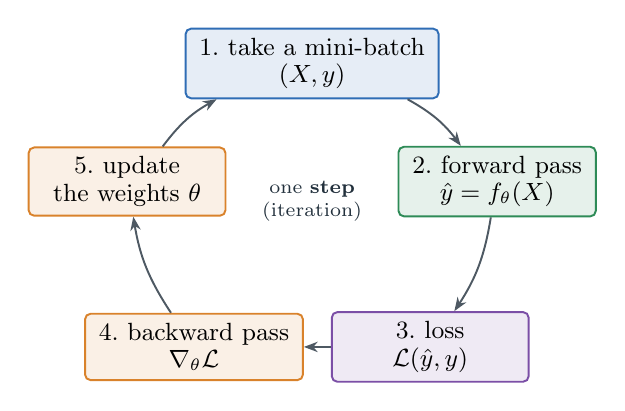
\begin{tikzpicture}[font=\footnotesize]
  \node[stage=cEmb,minimum width=25mm] (b) at (0,2.1) {1.\ take a mini-batch\\[-1pt]$(X,y)$};
  \node[stage=cFfn,minimum width=25mm] (f) at (2.35,0.6) {2.\ forward pass\\[-1pt]$\hat y=f_\theta(X)$};
  \node[stage=cOut,minimum width=25mm] (l) at (1.5,-1.5) {3.\ loss\\[-1pt]$\mathcal L(\hat y,y)$};
  \node[stage=cAtt,minimum width=25mm] (g) at (-1.5,-1.5) {4.\ backward pass\\[-1pt]$\nabla_\theta\mathcal L$};
  \node[stage=cAtt,minimum width=25mm] (u) at (-2.35,0.6) {5.\ update\\[-1pt]the weights $\theta$};
  \draw[flow] (b) to[bend left=12] (f); \draw[flow] (f) to[bend left=12] (l); \draw[flow] (l) -- (g);
  \draw[flow] (g) to[bend left=12] (u); \draw[flow] (u) to[bend left=12] (b);
  \node[note,text=cInk,align=center] at (0,0.35) {one \textbf{step}\\(iteration)};
\end{tikzpicture}

\vspace{1mm}
\[
  \boxed{\;\theta\;\leftarrow\;\theta-\eta\,\nabla_\theta\mathcal L\;}
\]
{\footnotesize \textbf{Gradient descent}: the gradient points uphill on the loss surface;
step the other way. $\eta$ is the learning rate.}
\column{0.50\textwidth}
\small
\begin{block}{In words}
\footnotesize\setlength{\leftmargini}{1.7em}
\begin{enumerate}
  \item Initialise the weights randomly.
  \item \textbf{For each epoch} (one full pass over the training set):
  \begin{itemize}
    \item shuffle the training rows and cut them into mini-batches;
    \item \textbf{for each mini-batch}: forward, loss, backward, update;
    \item measure the loss on the \emph{validation} set (no updates).
  \end{itemize}
  \item Stop when the validation loss has not improved for a while; keep the best weights.
  \item Evaluate once on the test set.
\end{enumerate}
\end{block}
\begin{itemize}\footnotesize
  \item \key{Step / iteration}: one weight update. \key{Epoch}: enough steps to see every
        training row once. 623 rows in batches of 32 = 20 steps per epoch.
  \item The four knobs of the loop get a slide each: the gradient (13), the learning rate (14),
        the update rule (15), the batch (16).
  \item Nothing in the loop depends on the task: swap the loss and the same code does
        classification or regression (\texttt{fit} in \texttt{train.py}).
\end{itemize}
\end{columns}
\end{frame}

% ====================================================================== 13
\begin{frame}{Backpropagation: which way should each weight move?}
\begin{columns}[T,onlytextwidth]
\column{0.49\textwidth}
\small
We need $\partial\mathcal L/\partial w$ for \emph{every} weight. The network is a chain of simple
steps, so the \textbf{chain rule} gives all of them in one backward sweep \cite{3}:
\begin{block}{Backward pass ($\delta^{\ell}$ = error signal at layer $\ell$)}
\vspace{-3mm}
\begin{align*}
 \delta^{L} &= \partial\mathcal L/\partial z^{L} && \text{from the loss (slide 11)}\\
 \delta^{\ell} &= \bigl(\delta^{\ell+1}\,W^{\ell+1\,\T}\bigr)\odot\phi'(z^{\ell}) && \text{send it back one layer}\\
 \frac{\partial\mathcal L}{\partial W^{\ell}} &= a^{\ell-1\,\T}\,\delta^{\ell},\qquad
 \frac{\partial\mathcal L}{\partial b^{\ell}}=\delta^{\ell} && \text{gradients}
\end{align*}
\end{block}
\begin{itemize}\footnotesize
  \item A weight's gradient = (activation feeding it) $\times$ (error at its output).
  \item Cost: about the same as one forward pass.
  \item PyTorch does this automatically (\texttt{loss.backward()}). \texttt{mlp\_numpy.py} does it
        by hand in about 15 lines and matches finite differences to $10^{-10}$.
\end{itemize}
\column{0.48\textwidth}
\small
\textbf{The network from slide 7} \ ($\hat y=2.5$, $y=2$, $\mathcal L=0.25$)
{\footnotesize
\begin{align*}
 \delta^{2} &= 2(\hat y-y)=\num{1.0}\\
 \partial\mathcal L/\partial W^{2} &= a^{1\,\T}\delta^{2}=(1.0,\;0)\\
 \delta^{1} &= (1.0)\,(2.0,\,-1.0)\odot(1,\,0)=(\num{2.0},\;0)\\
 \partial\mathcal L/\partial W^{1} &= x^{\T}\delta^{1}=
   \begin{bmatrix}1\\2\end{bmatrix}\begin{bmatrix}2&0\end{bmatrix}=\begin{bmatrix}2&0\\4&0\end{bmatrix}
\end{align*}}
{\footnotesize The switched-off neuron has $\phi'=0$: no gradient reaches its weights this time.}

\vspace{1mm}
\begin{block}{One update, two learning rates}
\footnotesize
\begin{tabular}{@{}lll@{}}
$\eta=0.01$: & $\hat y:\ 2.5\to2.24$ & loss $0.25\to\num{0.058}$ \ \ better\\
$\eta=0.1$: & $\hat y:\ 2.5\to0.40$ & loss $0.25\to{\color{cBad}\mathbf{2.56}}$ \ \ much worse
\end{tabular}

\vspace{1mm}
The gradient gives the \emph{direction}. It is only valid for a small step, so the step size
matters as much as the direction.
\end{block}
\end{columns}
\end{frame}

% ====================================================================== 14
\begin{frame}{The learning rate: the most important knob}
\begin{columns}[T,onlytextwidth]
\column{0.52\textwidth}
\centering
\begin{tikzpicture}
\begin{semilogyaxis}[width=8.6cm,height=5.5cm,xmin=0,xmax=60,ymin=0.05,ymax=1.6,
  xlabel={epoch},ylabel={training loss (MSE)},label style={font=\scriptsize},tick label style={font=\tiny},
  axis lines=left,ymajorgrids,grid style={cInk!10},log ticks with fixed point,ytick={0.05,0.1,0.2,0.5,1},
  legend columns=2,legend style={font=\scriptsize,draw=none,fill=none,at={(0.5,-0.24)},anchor=north,/tikz/every even column/.append style={column sep=3mm}},legend cell align=left,every axis plot/.append style={line width=1.1pt,no marks}]
  \addplot[cTok,dashed] table[x=epoch,y=Small]{generated/lr.dat}; \addlegendentry{$\eta=0.0005$: too slow}
  \addplot[cFfn] table[x=epoch,y=Good]{generated/lr.dat}; \addlegendentry{$\eta=0.02$: smooth}
  \addplot[cAtt,line width=0.8pt] table[x=epoch,y=Noisy]{generated/lr.dat}; \addlegendentry{$\eta=0.25$: erratic}
  \addplot[cBad] table[x=epoch,y=Broken]{generated/lr.dat}; \addlegendentry{$\eta=0.3$: stuck at 1.0}
\end{semilogyaxis}
\end{tikzpicture}

\vspace{-0.5mm}
{\scriptsize\color{cTok}Measured: Auto MPG, $10\to32\to32\to1$ network, plain SGD, batch 32, same initial weights.
One run per setting.}
\column{0.45\textwidth}
\small
The learning rate $\eta$ is the step length in $\theta\leftarrow\theta-\eta\,\nabla\mathcal L$.
\begin{itemize}
  \item \textbf{Too small} ($0.0005$): every step helps, but after 60 epochs the loss is still
        \lrSmallFinal.
  \item \textbf{About right} ($0.02$): fast, steady descent to \lrGoodFinal.
  \item \textbf{Large} ($0.25$): the loss jumps up and down. This run happened to end low
        (\lrNoisyFinal), but it is one small step from failure.
  \item \textbf{Too large} ($0.3$): an early step overshoots so far that the ReLU units switch
        off. The network then predicts the mean forever (loss 1.0 for a standardised target).
        At $\eta=0.35$ the weights overflow to NaN in the first epoch.
\end{itemize}
\begin{block}{Practice}
\footnotesize
Search on a log scale ($0.001,\,0.003,\,0.01,\dots$) and judge by \emph{validation} loss.
If the loss explodes or stalls at a round number, lower $\eta$ first. Many recipes also
shrink $\eta$ during training (a ``schedule'').
\end{block}
\end{columns}
\end{frame}

% ====================================================================== 15
\begin{frame}{Optimizers: smarter update rules}
\begin{columns}[T,onlytextwidth]
\column{0.49\textwidth}
\small
All use the same gradient $g=\nabla_\theta\mathcal L$ from a mini-batch; they differ in how it
becomes a step.

\vspace{1mm}
\key{SGD} (stochastic gradient descent) \cite{10}
\[ \theta\leftarrow\theta-\eta\,g \]
\key{Momentum} \cite{11}: keep a running velocity; steady directions build speed, zig-zags cancel.
\[ v\leftarrow\mu v+g,\qquad\theta\leftarrow\theta-\eta\,v\qquad(\mu=0.9) \]
\key{Adam} \cite{12}: momentum, plus a separate step size per weight from the running mean of $g^2$.
\vspace{-1mm}
\begin{align*}
 m &\leftarrow\beta_1m+(1-\beta_1)g, & v &\leftarrow\beta_2v+(1-\beta_2)g^2\\[-1pt]
 \theta &\leftarrow\theta-\eta\,\frac{\hat m}{\sqrt{\hat v}+\epsilon}
   & &(\hat m,\hat v:\text{ bias-corrected})
\end{align*}
\vspace{-4mm}

{\footnotesize Defaults $\beta_1=0.9$, $\beta_2=0.999$, $\eta=10^{-3}$. Each weight moves about
$\eta$ per step whatever the size of its gradient. \textbf{AdamW} \cite{13} adds weight decay
done correctly (slide 17).}
\column{0.48\textwidth}
\centering
\begin{tikzpicture}
\begin{loglogaxis}[width=8.2cm,height=5.2cm,xmin=0.0002,xmax=0.45,ymin=0.06,ymax=0.9,
  xlabel={learning rate $\eta$},ylabel={best validation loss},label style={font=\scriptsize},
  tick label style={font=\tiny},axis lines=left,ymajorgrids,grid style={cInk!10},
  log ticks with fixed point,ytick={0.07,0.1,0.2,0.4,0.8},xtick={0.0003,0.001,0.003,0.01,0.03,0.1,0.3},
  xticklabels={.0003,.001,.003,.01,.03,.1,.3},
  legend style={font=\scriptsize,draw=none,fill=none,at={(0.42,0.98)},anchor=north},legend cell align=left,
  every axis plot/.append style={line width=1.1pt,mark size=1.5pt}]
  \addplot[cTok,mark=*] table[x=lr,y=sgd]{generated/optgrid.dat}; \addlegendentry{SGD}
  \addplot[cAtt,mark=square*] table[x=lr,y=momentum]{generated/optgrid.dat}; \addlegendentry{momentum}
  \addplot[cFfn,mark=triangle*] table[x=lr,y=adam]{generated/optgrid.dat}; \addlegendentry{Adam}
\end{loglogaxis}
\end{tikzpicture}

\vspace{-0.5mm}
{\scriptsize\color{cTok}Measured: same network and data as slide 14, 60 epochs, one run per point.}

\raggedright\vspace{1mm}
{\footnotesize
\begin{itemize}
  \item \textbf{Tuned, they tie}: best loss \optSgdVal{} (SGD), \optMomentumVal{} (momentum),
        \optAdamVal{} (Adam) on this small problem.
  \item \textbf{Adam forgives a bad guess}: from $\eta=0.0003$ to $0.1$ its loss stays within
        \optAdamVal--\optAdamWorst; SGD ranges from \optSgdVal{} to \optSgdWorst.
  \item Hence the usual advice: start with Adam at $10^{-3}$; all three degrade sharply at $\eta=0.3$.
\end{itemize}}
\end{columns}
\end{frame}

% ====================================================================== 16
\begin{frame}{Batching: how many examples per update?}
\begin{columns}[T,onlytextwidth]
\column{0.50\textwidth}
\small
The true gradient averages over \emph{all} training rows. A \key{mini-batch} of $B$ rows gives a
cheap, noisy estimate of it; the noise shrinks like $1/\sqrt B$.

\vspace{1mm}
{\footnotesize
\renewcommand{\arraystretch}{1.2}
\begin{tabular}{@{}lp{58mm}@{}}
\toprule
$B=N$ & \textbf{full batch}: exact gradient, one update per epoch\\
$1<B<N$ & \textbf{mini-batch}: the standard choice, typically 16--256\\
$B=1$ & \textbf{stochastic}: one row per update; very noisy, no parallelism\\
\bottomrule
\end{tabular}}

\vspace{2mm}
\begin{itemize}\footnotesize
  \item \textbf{Why batches are fast}: a batch is a matrix $X\in\R^{B\times n}$, and $XW+b$
        processes all $B$ rows in one vectorised operation.
  \item \textbf{Shuffle every epoch} so batches differ and no ordering in the file (sorted by
        date, by class\dots) biases the updates.
  \item \textbf{Noise is not all bad}: it helps the weights escape poor regions, and small
        batches give many more updates per epoch.
  \item Batch size and learning rate interact: a larger batch gives a steadier gradient and
        usually tolerates (and needs) a larger $\eta$.
\end{itemize}
\column{0.47\textwidth}
\centering
\begin{tikzpicture}
\begin{semilogyaxis}[width=7.9cm,height=4.5cm,xmin=0,xmax=60,ymin=0.07,ymax=1.2,
  xlabel={epoch},ylabel={validation loss},label style={font=\scriptsize},tick label style={font=\tiny},
  axis lines=left,ymajorgrids,grid style={cInk!10},log ticks with fixed point,ytick={0.1,0.2,0.5,1},
  legend style={font=\scriptsize,draw=none,fill=none,at={(0.98,0.98)},anchor=north east},legend cell align=left,
  legend columns=2,every axis plot/.append style={line width=1.1pt,no marks}]
  \addplot[cBad] table[x=epoch,y=bOne]{generated/batch.dat}; \addlegendentry{$B=1$}
  \addplot[cAtt] table[x=epoch,y=bEight]{generated/batch.dat}; \addlegendentry{$B=8$}
  \addplot[cFfn] table[x=epoch,y=bThirtyTwo]{generated/batch.dat}; \addlegendentry{$B=32$}
  \addplot[cTok,dashed] table[x=epoch,y=bFull]{generated/batch.dat}; \addlegendentry{$B=\mpgNtrain$ (full)}
\end{semilogyaxis}
\end{tikzpicture}

{\footnotesize
\begin{tabular}{@{}rrrr@{}}
\toprule
batch $B$ & updates/epoch & ms/epoch & val.\ loss, 60 epochs\\
\midrule
1 & \bsOneUpdates & \bsOneMs & \bsOneVal\\
8 & \bsEightUpdates & \bsEightMs & \bsEightVal\\
32 & \bsThirtyTwoUpdates & \bsThirtyTwoMs & \bsThirtyTwoVal\\
\mpgNtrain & \bsFullUpdates & \bsFullMs & \bsFullVal\\
\bottomrule
\end{tabular}}

\vspace{1mm}
{\scriptsize\color{cTok}Measured: Auto MPG (\mpgNtrain{} training rows), SGD, $\eta=0.02$, one run each, 2 CPU cores.
Per epoch, small batches learn more but cost far more time.}
\end{columns}
\end{frame}

% ====================================================================== 17
\begin{frame}{Overfitting: when the training loss lies}
\begin{columns}[T,onlytextwidth]
\column{0.50\textwidth}
\centering
\begin{tikzpicture}
\begin{axis}[width=8.4cm,height=5.4cm,xmin=0,xmax=150,ymin=0,ymax=1.4,
  xlabel={epoch},ylabel={loss (cross-entropy)},label style={font=\scriptsize},tick label style={font=\tiny},
  axis lines=left,ymajorgrids,grid style={cInk!10},
  legend style={font=\scriptsize,draw=none,fill=none,at={(0.12,0.99)},anchor=north west},legend cell align=left,
  every axis plot/.append style={line width=1.1pt,no marks}]
  \addplot[cEmb] table[x=epoch,y=train]{generated/overfit.dat}; \addlegendentry{training loss}
  \addplot[cAtt] table[x=epoch,y=val]{generated/overfit.dat}; \addlegendentry{validation loss}
  \draw[cInk,dashed] (axis cs:\ofBestEpoch,0) -- (axis cs:\ofBestEpoch,1.25);
  \node[font=\tiny,anchor=west,text=cInk] at (axis cs:28,0.42) {validation loss is lowest at epoch \ofBestEpoch{} (dashed line)};
\end{axis}
\end{tikzpicture}

\vspace{-0.5mm}
{\scriptsize\color{cTok}Measured: Titanic, deliberately oversized $15\to256\to256\to2$ network
(\ofParams{} weights for 623 training rows), Adam, no regularisation.}

\vspace{1.5mm}
\raggedright\small
Training loss keeps falling to \ofLastTrain; validation loss bottoms out at \ofBestVal{} and climbs
to \ofLastVal. The network is \textbf{memorising} training rows, noise included, instead of learning
the pattern.
\column{0.47\textwidth}
\small
\begin{block}{Diagnosis}
\footnotesize
Always plot both curves. A widening gap between training and validation loss is overfitting.
Both high and flat is \emph{under}fitting: the model is too small, or $\eta$ is wrong.
\end{block}
\textbf{Remedies}, roughly in order of cost:
\begin{itemize}\footnotesize
  \item \key{Early stopping} \cite{15}: keep the weights from the best validation epoch
        (\texttt{-{}-patience}). Here test accuracy is \ofStoppedAcc\% with it,
        \ofLastAcc\% when trained to the end.
  \item \key{Weight decay}: shrink every weight slightly each step, $\theta\leftarrow\theta-\eta\lambda\theta$,
        so the fit stays smooth (\texttt{-{}-weight\_decay}).
  \item \key{Dropout} \cite{14}: during training, zero a random fraction of hidden activations each
        step so no neuron can rely on another (\texttt{-{}-dropout}).
  \item \key{A smaller network}: fewer weights, less room to memorise.
  \item \key{More data}: the only remedy that also makes the model better.
\end{itemize}
{\footnotesize Rule of thumb: pick a network big enough to overfit, then regularise it back.}
\end{columns}
\end{frame}

% ====================================================================== 18
\begin{frame}[fragile]{Code: the model and the training loop in PyTorch}
\vspace{-1mm}
{\footnotesize \texttt{mlp.py}: build the stack of layers from a list such as \texttt{hidden=[32, 32]}}
\lstinputlisting[style=py,basicstyle=\ttfamily\fontsize{5.7}{6.8}\selectfont,linerange={19-22,25-27}]{../mlp.py}
\vspace{0.5mm}
{\footnotesize \texttt{train.py}, inside \texttt{fit()}: the loop of slide 12, with validation and early stopping (lines verbatim; logging and dropout omitted)}
\lstinputlisting[style=py,basicstyle=\ttfamily\fontsize{5.7}{6.8}\selectfont,linerange={85-92,94-96,101-106,109}]{../train.py}
\vspace{-0.5mm}

\end{frame}

% ====================================================================== 19
\begin{frame}{The harness on real data: train, validate, test}
\begin{columns}[T,onlytextwidth]
\column{0.49\textwidth}
\small
\textbf{Classification}: \texttt{python train.py -{}-task titanic}

\vspace{1mm}
\begin{minipage}[c]{0.44\textwidth}
\centering
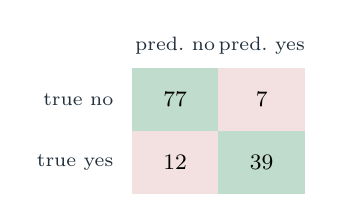
\begin{tikzpicture}[x=11mm,y=8mm,font=\footnotesize]
  \node[fill=cFfn!30,minimum width=11mm,minimum height=8mm] at (0,1) {\cmTN};
  \node[fill=cBad!15,minimum width=11mm,minimum height=8mm] at (1,1) {\cmFP};
  \node[fill=cBad!15,minimum width=11mm,minimum height=8mm] at (0,0) {\cmFN};
  \node[fill=cFfn!30,minimum width=11mm,minimum height=8mm] at (1,0) {\cmTP};
  \node[note,text=cInk] at (0,1.85) {pred.\ no}; \node[note,text=cInk] at (1,1.85) {pred.\ yes};
  \node[note,text=cInk,anchor=east] at (-0.6,1) {true no}; \node[note,text=cInk,anchor=east] at (-0.6,0) {true yes};
\end{tikzpicture}
\end{minipage}\hfill
\begin{minipage}[c]{0.54\textwidth}
\footnotesize
\titanicNtest{} test passengers, split 0:\\
accuracy \textbf{\titanicSeedAcc\%}\\
majority baseline \titanicBaseAcc\%\\
$15\to32\to32\to2$, \titanicMlpParams{} weights, stopped after \titanicMlpEpochs{} epochs
\end{minipage}

\vspace{2mm}
{\footnotesize
\begin{tabular}{@{}lcc@{}}
\toprule
test accuracy, 10 random splits & mean & std\\
\midrule
MLP (32, 32) & \titanicMlpMean\% & \titanicMlpStd\\
no hidden layer (logistic regression) & \titanicLinearMean\% & \titanicLinearStd\\
\bottomrule
\end{tabular}}

\vspace{1.5mm}
{\footnotesize \textbf{Honest reading}: both models clearly beat the baseline, but the hidden layers add
nothing here. The MLP wins on only \titanicMlpBetter{} of 10 splits. A single split
(\titanicSeedAcc\%) can flatter either model: with \titanicNtest{} test rows, one standard error is
about 3 points.}
\column{0.48\textwidth}
\small
\textbf{Regression}: \texttt{python train.py -{}-task mpg}

\vspace{0.5mm}
\begin{minipage}[c]{0.50\textwidth}
\begin{tikzpicture}
\begin{axis}[width=4.7cm,height=4.7cm,xmin=8,xmax=48,ymin=8,ymax=48,
  xlabel={true mpg},ylabel={predicted mpg},label style={font=\tiny},tick label style={font=\tiny},
  xtick={10,20,30,40},ytick={10,20,30,40},ylabel shift=-3pt]
  \addplot[cInk!50,dashed,domain=8:48,samples=2] {x};
  \addplot[only marks,mark size=1pt,cOut] table[x=true,y=pred]{generated/mpg_scatter.dat};
\end{axis}
\end{tikzpicture}
\end{minipage}\hfill
\begin{minipage}[c]{0.47\textwidth}
\footnotesize\raggedright
\mpgNtest{} test cars, split 0:\\
RMSE \textbf{\mpgSeedRmse{} mpg}\\
MAE \mpgSeedMae{} mpg, \ $R^2=\mpgSeedRsq$\\
predict-the-mean baseline: RMSE \mpgBaseRmse
\end{minipage}

\vspace{1mm}
{\footnotesize
\begin{tabular}{@{}lcc@{}}
\toprule
test RMSE (mpg), 10 random splits & mean & std\\
\midrule
MLP (32, 32) & \mpgMlpMean & \mpgMlpStd\\
no hidden layer (linear regression) & \mpgLinearMean & \mpgLinearStd\\
\bottomrule
\end{tabular}}

\vspace{1.5mm}
{\footnotesize \textbf{Here the hidden layers help}: fuel economy bends with weight and power, and the MLP is
better on \mpgMlpBetter{} of 10 splits. The lesson: always run the linear baseline (\texttt{-{}-hidden} with no
sizes). On small tables, tree ensembles are often stronger still \cite{17}.}
\end{columns}
\end{frame}

% ====================================================================== 20
\begin{frame}{References and how to run the code}
\fontsize{6.4}{7.9}\selectfont
\begin{columns}[T,onlytextwidth]
\column{0.49\textwidth}
\begin{enumerate}[{[1]}]\setlength{\itemsep}{0.6pt}
\item Rosenblatt. \emph{The Perceptron: A Probabilistic Model for Information Storage and Organization in the Brain.} Psychological Review 65(6), 1958.
\item Minsky, Papert. \emph{Perceptrons.} MIT Press, 1969.
\item Rumelhart, Hinton, Williams. \emph{Learning Representations by Back-propagating Errors.} Nature 323, 1986.
\item Cybenko. \emph{Approximation by Superpositions of a Sigmoidal Function.} Mathematics of Control, Signals and Systems 2, 1989.
\item Hornik, Stinchcombe, White. \emph{Multilayer Feedforward Networks are Universal Approximators.} Neural Networks 2, 1989.
\item Nair, Hinton. \emph{Rectified Linear Units Improve Restricted Boltzmann Machines.} ICML 2010.
\item Glorot, Bengio. \emph{Understanding the Difficulty of Training Deep Feedforward Neural Networks.} AISTATS 2010.
\item He, Zhang, Ren, Sun. \emph{Delving Deep into Rectifiers.} ICCV 2015. arXiv:1502.01852
\item LeCun, Bottou, Orr, M\"uller. \emph{Efficient BackProp.} In Neural Networks: Tricks of the Trade, Springer, 1998.
\item Robbins, Monro. \emph{A Stochastic Approximation Method.} Annals of Mathematical Statistics 22, 1951.
\item Polyak. \emph{Some Methods of Speeding up the Convergence of Iteration Methods.} USSR Computational Mathematics and Mathematical Physics 4(5), 1964.
\item Kingma, Ba. \emph{Adam: A Method for Stochastic Optimization.} ICLR 2015. arXiv:1412.6980
\end{enumerate}
\column{0.49\textwidth}
\begin{enumerate}[{[1]}]\setlength{\itemsep}{0.6pt}
\setcounter{enumi}{12}
\item Loshchilov, Hutter. \emph{Decoupled Weight Decay Regularization.} ICLR 2019. arXiv:1711.05101
\item Srivastava, Hinton, Krizhevsky, Sutskever, Salakhutdinov. \emph{Dropout: A Simple Way to Prevent Neural Networks from Overfitting.} JMLR 15, 2014.
\item Prechelt. \emph{Early Stopping -- But When?} In Neural Networks: Tricks of the Trade, Springer, 1998.
\item Goodfellow, Bengio, Courville. \emph{Deep Learning.} MIT Press, 2016. deeplearningbook.org
\item Grinsztajn, Oyallon, Varoquaux. \emph{Why Do Tree-based Models Still Outperform Deep Learning on Typical Tabular Data?} NeurIPS 2022. arXiv:2207.08815
\item Paszke et al. \emph{PyTorch: An Imperative Style, High-Performance Deep Learning Library.} NeurIPS 2019. arXiv:1912.01703
\item Data: Titanic and Auto MPG tables as distributed in \emph{seaborn-data} (github.com/mwaskom/seaborn-data); Auto MPG is from the UCI Machine Learning Repository.
\end{enumerate}

\vspace{0.5mm}
{\fontsize{6.6}{8.1}\selectfont\color{cInk}
\textbf{Run it} (Python, NumPy, PyTorch; about a minute on a laptop CPU)

\vspace{0.5mm}
\begin{tabular}{@{}l>{\raggedright\arraybackslash}p{40mm}@{}}
\texttt{python test\_mlp.py} & six checks, incl.\ backprop vs.\ finite differences\\
\texttt{python walkthrough.py} & the hand calculations (slides 3, 7--9, 11, 13)\\
\texttt{python mlp\_numpy.py} & from-scratch network learns XOR\\
\texttt{python train.py -{}-task titanic} & the harness; \texttt{-{}-help} lists every knob\\
\texttt{python experiments.py} & figures for slides 6, 14--17, 19\\
\end{tabular}

\vspace{1mm}
\textbf{Exercises.} Feed the leaky \texttt{survived} column in and watch accuracy hit 100\%.
Remove standardisation and retrain. Replace ReLU by sigmoid in a 6-layer network.}
\end{columns}
\end{frame}

\end{document}
